\documentclass[../main.tex]{subfiles}

\begin{document}
	
	В данном разделе приведены характеристики оборудования на котором производилось тестирование. 
	Описаны параметры тестирования. 
	Проводятся результаты измерений.
	
\subsection{Характеристики оборудования}

	\begin{enumerate}[1)]
		\item Компьютер:
		\begin{enumerate}
			\item Тип компьютера   Компьютер с ACPI на базе x64;
			\item Операционная система   Microsoft Windows 10 Pro.
		\end{enumerate}
		\item Системная плата:
		\begin{enumerate}
			\item тип ЦП   DualCore Intel Core i5-6200U, 2700 MHz (27 x 100);
			\item системная плата   HP 8079;
			\item чипсет системной платы   Intel Sunrise Point-LP, Intel Skylake-U;
			\item системная память   8072 МБ (DDR4 SDRAM).
		\end{enumerate}
	\end{enumerate}

\subsection{Результаты замеров}

	В данном подразделе приведены результаты замеров в таблицу \ref{tab:2}. Представлен график зависимости времени от количества слов \ref{fig:graph}
	
	Замеры проводились по следующим параметрам:
	
	\begin{enumerate}[1)]
		\item Количество итераций: 1000;
		\item Количество слов: 10 - 10000;
		\item Длинна слов: Фиксированная, 10 символов
	\end{enumerate}

	\begin{table}
		\label{tab:2}
		\begin{tabular}{|c|c|c|r|}
			\hline
			& \multicolumn{ 2}{|c|}{Способ реализации} &            \\
			\hline
			Количество слов & Последовательный & Конвеерный  &       diff \\
			\hline
			10 &      0,109 &      0,110 &      0,991 \\
			\hline
			100 &      0,938 &      0,922 &      1,017 \\
			\hline
			200 &      1,766 &      2,094 &      0,843 \\
			\hline
			300 &      3,047 &      2,813 &      1,083 \\
			\hline
			400 &      3,609 &      3,953 &      0,913 \\
			\hline
			500 &      4,328 &      4,578 &      0,945 \\
			\hline
			600 &      5,344 &      5,703 &      0,937 \\
			\hline
			700 &      6,594 &      6,282 &      1,050 \\
			\hline
			800 &      7,782 &      6,860 &      1,134 \\
			\hline
			900 &      8,200 &      6,860 &      1,195 \\
			\hline
			1000 &      9,687 &      8,829 &      1,097 \\
			\hline
			2000 &     17,687 &     17,125 &      1,033 \\
			\hline
			3000 &     27,297 &     25,531 &      1,069 \\
			\hline
			4000 &     37,000 &     34,578 &      1,070 \\
			\hline
			5000 &     49,031 &     42,469 &      1,155 \\
			\hline
			6000 &     54,859 &     53,984 &      1,016 \\
			\hline
			7000 &     64,094 &     59,750 &      1,073 \\
			\hline
			8000 &     73,375 &     68,859 &      1,066 \\
			\hline
			9000 &     82,344 &     78,672 &      1,047 \\
			\hline
			10000 &     99,311 &     86,344 &      1,150 \\
			\hline
		\end{tabular} 
		\caption{Таблицы измерений}
	\end{table} 

	\begin{figure}[H]
		\centering
		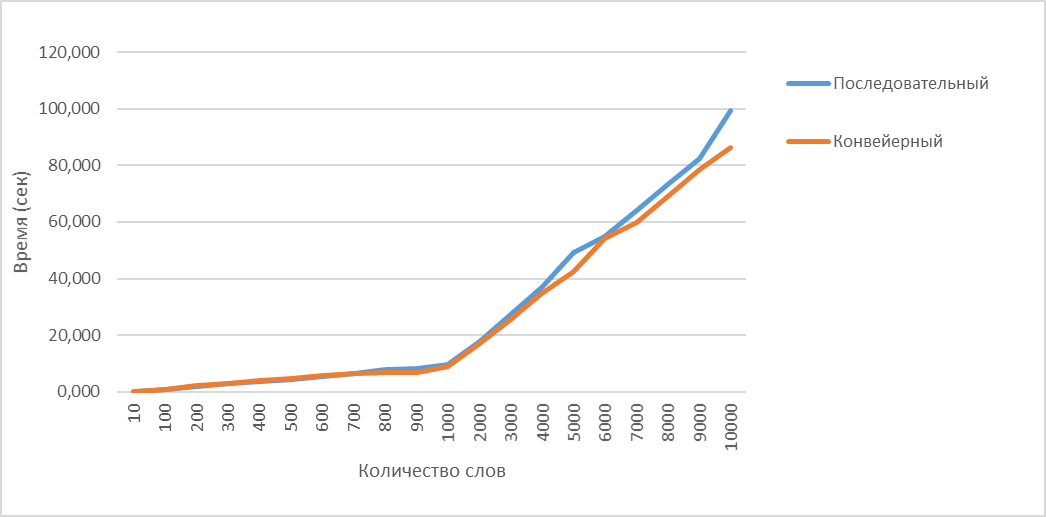
\includegraphics[scale=0.5]{src/img/График}
		\caption{График зависимости времени от количества слов}
		\label{fig:graph}
	\end{figure}

	Не смотря на то что вычисляемая задача требовала минимальных вычислительных мощностей, мы можем видеть, что конвейерный подход, на количестве слов большее 2000 начинает показывать производительность лучше, чем классический последовательный метод реализации (хоть и достаточно маленькую в 1.033).
	
\subsection{Вывод}

	В данном разделе приведены характеристики оборудования на котором проводилось тестирование
	Указаны результаты замеров эффективности 2 подходов к выполнению задачи.

\end{document}